\section{Espacios Tangentes}
\begin{frame}
	\frametitle{Espacios tangentes en $\R^n$}
	\begin{definition}[Vectores y Espacios Tangentes en $\R^n$]\label{Definición: Espacio Tangente en Rn}
		Sea $a$ un punto en $\R^n$, definiremos el \textbf{espacio tangente a $\R^n$ en el punto $a$} como el conjunto:
		\[ T_{a}(\mathbb{R}^{n}) = \{a\} \times \R^n = \{(a,v): v \in \R^n\} \]

		Un \bf{vector tangente} a $\R^n$ es un elemento de $T_a(\R^n)$ para algún $a \in \R^n$.
	\end{definition}\pause

	$T_a(\R^n)$ tiene estructura de espacio vectorial. Dados $a \in \mathbb{R}^{n}$, $c \in \mathbb{R}$ y $v_a, w_a \in T_a(\mathbb{R}^n)$:
	\begin{align*}
		v_a + w_a & = (v+w)_a \\
		c(v_a)    & = (cv)_a
	\end{align*}
\end{frame}

\begin{frame}
	\frametitle{Ejemplo de espacios tangentes}
	\begin{columns}[t]
		\column{.5\textwidth}
		\centering
		\begin{figure}
			\vspace{-12pt}
			\scalebox{.4}{\begin{tikzpicture}
\draw[thick,->] (-0.5,0) -- (5,0) node[anchor=west]{$x$};
\draw[thick,->] (0,-0.5) -- (0,5) node[anchor=south]{$y$};

\draw (0.5,0.5) rectangle (4,4);
\node at (4.5,4.5) {$T_a(\R^n)$};

\draw[thick,->] (1,1.5) -- (3.5,1.5);
\draw[thick,->] (1.5,1) -- (1.5,3.5);
\filldraw (1.5,1.5) circle (0.1);
\node at (1,1) {$a$};
\draw[thick, ->] (1.5,1.5) -- (3,2.75);
  \node at (3.25,2.5) {$v_a$};
\end{tikzpicture}

}\\
			\caption{Espacio tangente a un punto \\ en el plano.}
		\end{figure}
		\begin{figure}
			\vspace{-12pt}
			\scalebox{.4}{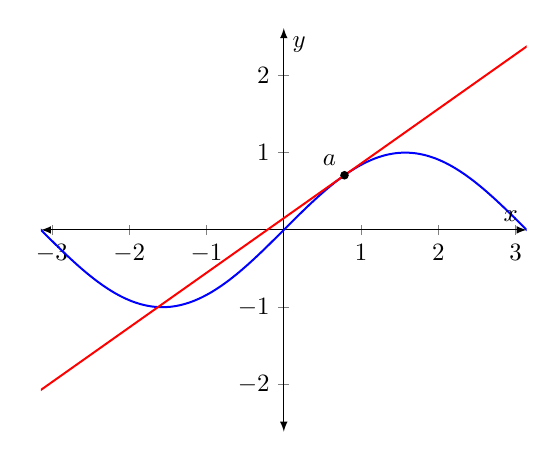
\begin{tikzpicture}[scale=0.90]
	\begin{axis}[
			% grid=both,
			xmin=-pi,
			xmax=pi,
			ymin=-1.6,
			ymax=1.6,
			axis lines=middle,
			xlabel = $x$,
			ylabel = $y$,
			axis line style={latex-latex},
      axis equal,
		]

		\addplot[
			samples=200,
			domain=-4*pi:4*pi,
			color=blue,
			thick,
			smooth,
		]
		{sin(deg(x))};

		\addplot[
			domain=-5:5,
			color=red,
      thick,
		]{( (sqrt(2) / 2) * (x - (pi/4)) ) +  (sqrt(2) / 2)};

		\addplot+[
			mark options={black},
      mark size=1.5pt,
		] coordinates {(0.785398,0.707106)} node [black, left=6pt, above=0.5pt] {$a$};
	\end{axis}
\end{tikzpicture}

}\\
			\caption{Espacio tangente a un punto \\ de $\sin(x)$.}
		\end{figure}
		\column{.5\textwidth}
		\centering
		\begin{figure}
			\scalebox{.5}{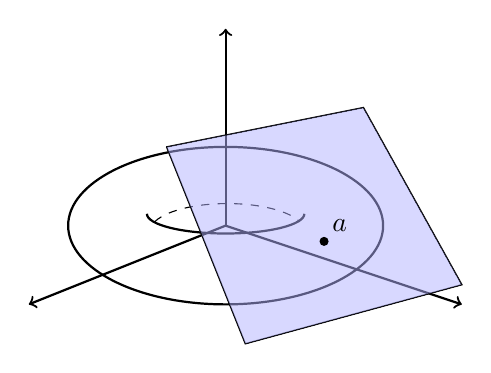
\begin{tikzpicture}

	% Ejes R3
	\draw [thick,->] (0,0) -- (0,2.5);
	\draw [thick,->] (0,0) -- (3,-1);
	\draw [thick,->] (0,0) -- (-2.5,-1);

	% Toro
	\draw [thick] (0,0) ellipse  (2 and 1);
	\draw [thick] (-1.0,0.15) arc (0:-180:-1.0 and 0.25);
  \draw [dashed] (-0.90,0.05) arc (20:160:-0.98 and 0.35);

  % Plano tangente
  \draw [line width=0.5] (-0.75,1) -- (1.75,1.5) -- (3,-0.75) -- (0.25,-1.5) -- (-0.75,1);
  \draw [fill=blue!30!white,opacity=0.5, line width=0] (-0.75,1) -- (1.75,1.5) -- (3,-0.75) -- (0.25,-1.5) -- (-0.75,1);

  % Punto $a$
	\filldraw (1.25,-0.2) circle (0.05);
	\node at (1.45,0) {$a$};
\end{tikzpicture}
}\\
			\caption{Espacio tangente a un punto \\ del $2-$toro.}
		\end{figure}
		\begin{figure}
			\vspace{-12pt}
			\scalebox{.45}{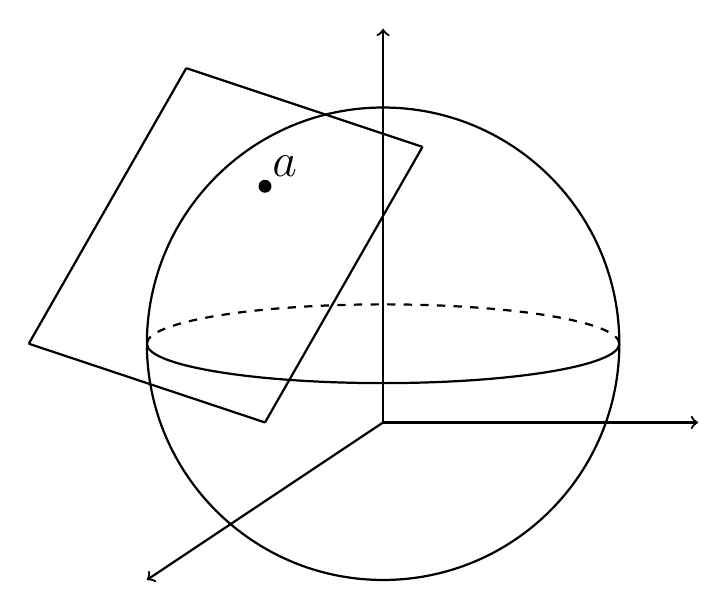
\begin{tikzpicture}
  % Esfera
  \draw [thick] (3,0) arc (0:180:3 and -0.5);
  \draw [thick, dashed] (-3,0) arc (180:0:3 and 0.5);
  \draw [thick] (0,0) circle (3);

  % Ejes R3
  \draw [thick,->] (0,-1) -- (0,4);
  \draw [thick,->] (0,-1) -- (4,-1);
  \draw [thick,->] (0,-1) -- (-3,-3);


  % Rectángulo (Espacio Tangente)
  \filldraw (-1.5,2) circle (0.075);
  \node[font=\fontsize{18pt}{18pt}] at (-1.25,2.25) {$a$};
  \draw [thick] (-2.5,3.5) -- (0.5,2.5);
  \draw [thick] (-2.5,3.5) -- (-4.5,0);
  \draw [thick] (-4.5,0) -- (-1.5,-1);
  \draw [thick] (0.5,2.5) -- (-1.5,-1);
\end{tikzpicture}
}\\
			\caption{Espacio tangente a un punto \\ de la $2-$esfera.}
		\end{figure}
	\end{columns}
\end{frame}

\begin{frame}
	\frametitle{Derivada direccional}
	Si tenemos un punto $a = (a_1, \dots, a_n) \in \R^n$ y un vector $v = \begin{bmatrix} v_1 \dots v_n \end{bmatrix} \in T_a(\mathbb{R}^{n})$ podemos parametrizar la recta que pasa por $a$ con dirección $v$ de la siguiente manera:

	\[\gamma(t) = (a_1 + tv_1, \dots, a_n + tv_n) \]
	\pause
	Si $f: \R^n \to \R$ es una función suave definida en una vecindad de $a$ y $v$ es un vector en $T_a(\R^n)$ podemos obtener la \textit{derivada direccional} de $f$ en $a$ en la dirección de $v$ como:
	\[
		D_v f = \left. \frac{d}{dt}\right|_{t=0} f(\gamma(t))
		= \sum_{i=1}^{n} v_i \left. \frac{\partial f}{\partial x_i} \right|_{a}
	\]
\end{frame}

\begin{frame}
	\frametitle{Derivada direccional}
	La derivada direccional es lineal y cumple la regla del producto. Esto quiere decir que si $f$ y $g$ son funciones suaves definida en una vecindad de $a \in \R^n$, $c$ es una constante y $v \in T_{a}(\R^n)$, entonces:
	\begin{itemize}
		\item $D_v(f+g) = D_v(f) + D_v(g)$
		\item $D_v(cf) = cD_v(f)$
		\item $D_v(fg) = f(a)D_v(g) + g(a)D_v(f)$
	\end{itemize} \pause

	\begin{definition}[Derivación en un punto]
		Si $a$ es un punto en $\R^n$ y $\omega: C^{\infty}(\R^{n}) \to \R$ es un funcional lineal, diremos que $\omega$ es una \textbf{derivación} en $a$ si cumple la regla del producto. 
	\end{definition}
\end{frame}

\begin{frame}
	\frametitle{Derivaciones}
	El conjunto de todas las derivaciones en $a$, al cual denotamos por $\mathcal{D}_a(\R^n)$, es un espacio vectorial bajo las operaciones:
	\begin{align*}
		(\omega_1 + \omega_2)(f) & = \omega_1(f) + \omega_2(f) \\
		(c\omega)(f)             & = c(\omega(f))
	\end{align*} \pause

	\begin{theorem}
		Los espacios $T_a(\R^n)$ y $\mathcal{D}_a(\R^n)$ son isomorfos y el isomorfismo está dado por:
		\begin{align*}
			\phi: T_a(\R^n) & \to \mathcal{D}_a(\R^n)                                                         \\
			v               & \mapsto D_v = \sum_{i=1}^n v_i \left. \frac{\partial}{\partial x_i} \right|_{a}
		\end{align*}
	\end{theorem}
\end{frame}

\begin{frame}
	\frametitle{Espacios tangentes a variedades}
	\begin{definition}[Derivación en un punto de una variedad]
		Sea $M$ una variedad suave y sea $p \in M$ un punto. Diremos que un mapa $\omega: C^{\infty}(M) \to \R$ es una \textbf{derivación} en $p$ si es lineal y además cumple la regla del producto.

		Llamaremos al conjunto de todas las derivaciones en un punto de una variedad el \textbf{espacio tangente} a la variedad en ese punto, este se denota $T_{p}M$.
	\end{definition}
\end{frame}

\begin{frame}
	\frametitle{Base para el espacio tangente}
	Si $M$ es una variedad suave $n-$dimensional, $p$ un punto en $M$ y $(U,\phi)$ una carta suave que contiene a $p$, $f: M \to \mathbb{R}^{n}$ una función suave definida en una vecindad de $p$ podemos definir:
	\[
		\partial \phi_{i} \big|_{p} (f)= 
		\left. \frac{\partial}{\partial \phi_{i}} \right|_{p} f
		= \left. \frac{\partial}{\partial x_{i}} \right|_{\phi(p)} (f \circ \phi^{-1})
	\]\pause

	\begin{theorem}[Base para el espacio tangente]
		Sean $M$ una variedad suave, $p \in M$ y $(U,\phi)$ una carta suave que contenga a $p$. El conjunto
		\[
			\partial \phi_{1} \big|_{p},
			\ldots,
			\partial \phi_{n} \big|_{p}
		\]
		forma una base para el espacio tangente $T_{p}M$.
	\end{theorem}

\end{frame}
